\chapter{Results}

  The reference image used for these results is Horse form the Shapes Repository
  \cite{horse}.  This is a fully connected mesh with 59547 edges, 39698 faces
  and 19851 vertices.

  The results of the two error metrics are presented below.  Figure
  \ref{simplification} shows the results of applying both error metrics to the
  model 3 times reducing the number of polygons by 50\% each time.  Both models
  are decent at 50\% polygon reduction. The simple error metric has produced a
  lot more obvious deformities, but it would be good enough for use with a nice
  normal map.  After removing another 50\% of the polygons however the story has
  changed a bit.  There are a lot of obvious deformities introduced in the legs
  of the horse especially.  These are likely the result of the very simple
  local curvature check that is performed, the angle across the single edge will
  be very small but between one of those triangles and the next will be large.

  Finally by only 12.5\% of the polygons remaining the model is horribly
  deformed (Fig. \ref{simple3}).  The error metric is obviously far too
  simplistic when compared to the Stan Melax's error metric's model at the same
  polygon level.

  Figure \ref{extreme} then shows the results of applying Stan Melax's error
  metric another 3 times, reducing the number of polygons to 50\% then to 25\%
  the next two times.  Alongside these it shows the image with a pre-calculated
  normal map added. The results shown here are quite impressive, at only 6.2\%
  of the original polygons the model is still very well rendered with flat
  shading and only has a slight loss of muscle definition when normal mapped.
  The biggest differences are around the nose and eyes, very high detail areas
  that would have had most of the detail destroyed to get to such a low polygon
  count.

  Even with over 98\% of the polygons removed the model is still quite
  recognisably a horse.  It even still has recognisable calfs and ears.  Once we
  reduce the model down to 0.4\% of the initial polygons the shape is mostly
  gone.  It is still recognisable as a four legged animal but exactly what it is
  is almost impossible to guess.  This level of detail is probably too low for
  use as anything but a very long distance model in any modern graphics
  application.  The 618 polygon model with normal map and an applied texture
  however could still be useful as a long distance low fidelity model.

  \begin{figure}
    \centering
    \subfloat[Initial Model - 39698 polygons - 100\%]{
      \label{initial}
      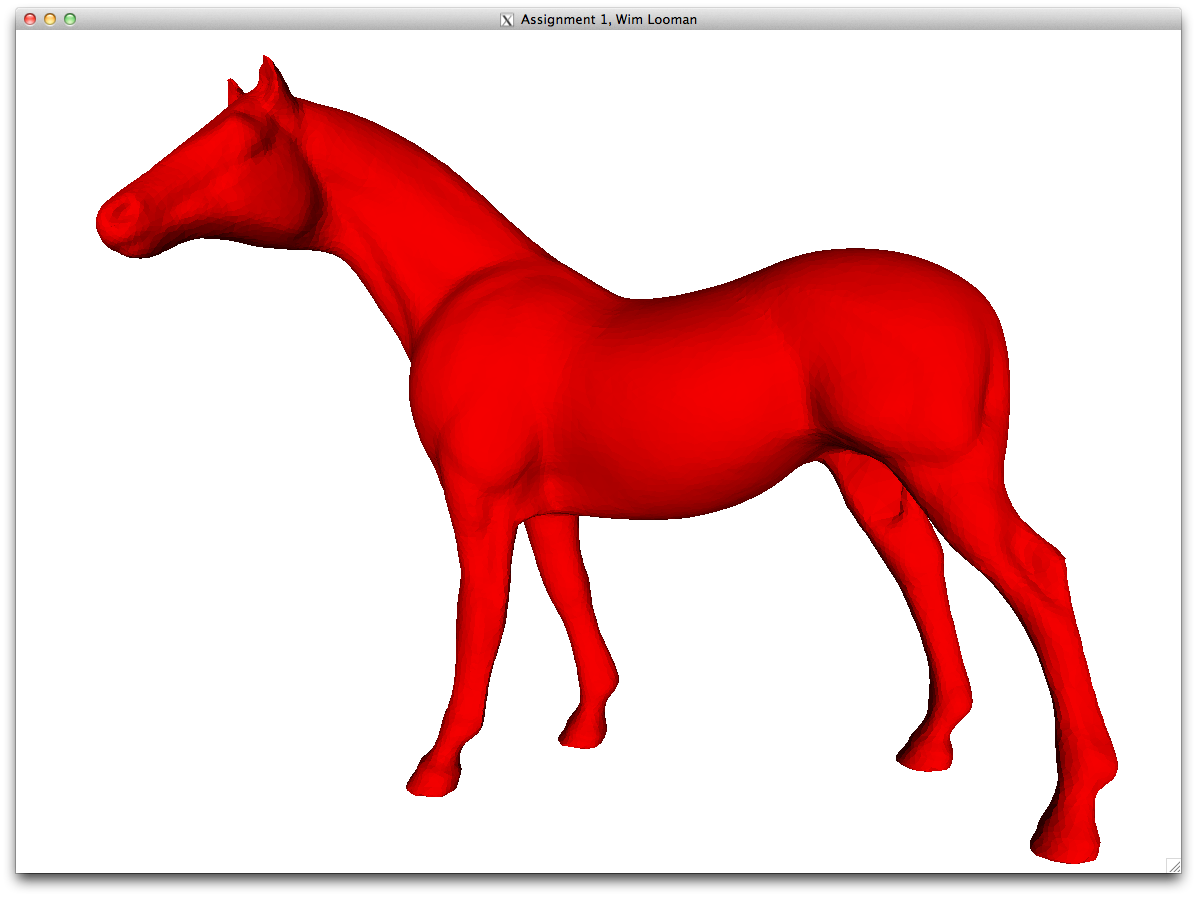
\includegraphics[width=0.35\textwidth]{images/Base_39698}
    }
    \\
    \subfloat[Simple Error Metric - 19848 polygons - 50\%]{
      \label{simple1}
      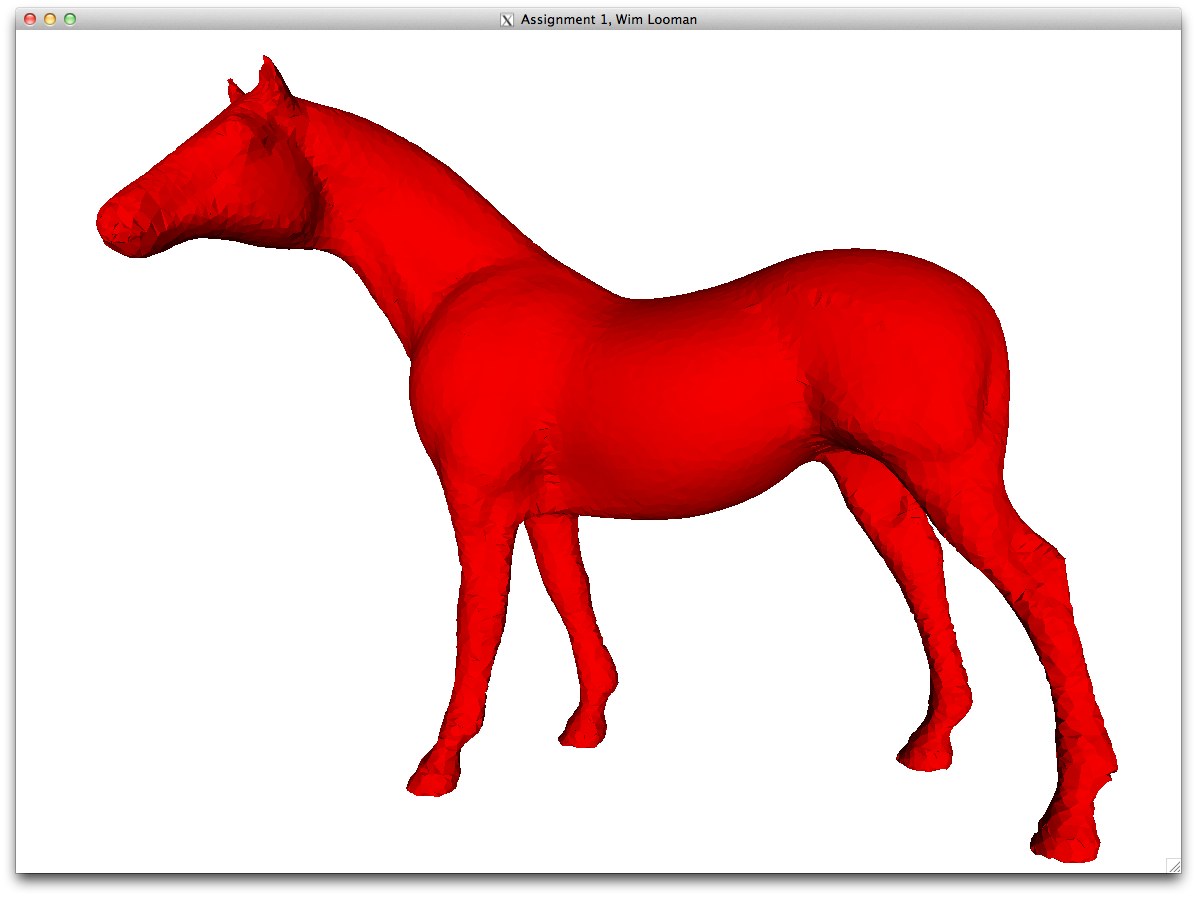
\includegraphics[width=0.35\textwidth]{images/Simple_19848}
    }
    \hspace{0.1\textwidth}
    \subfloat[Stan Melax's Error Metric - 19848 polygons - 50\%]{
      \label{melax1}
      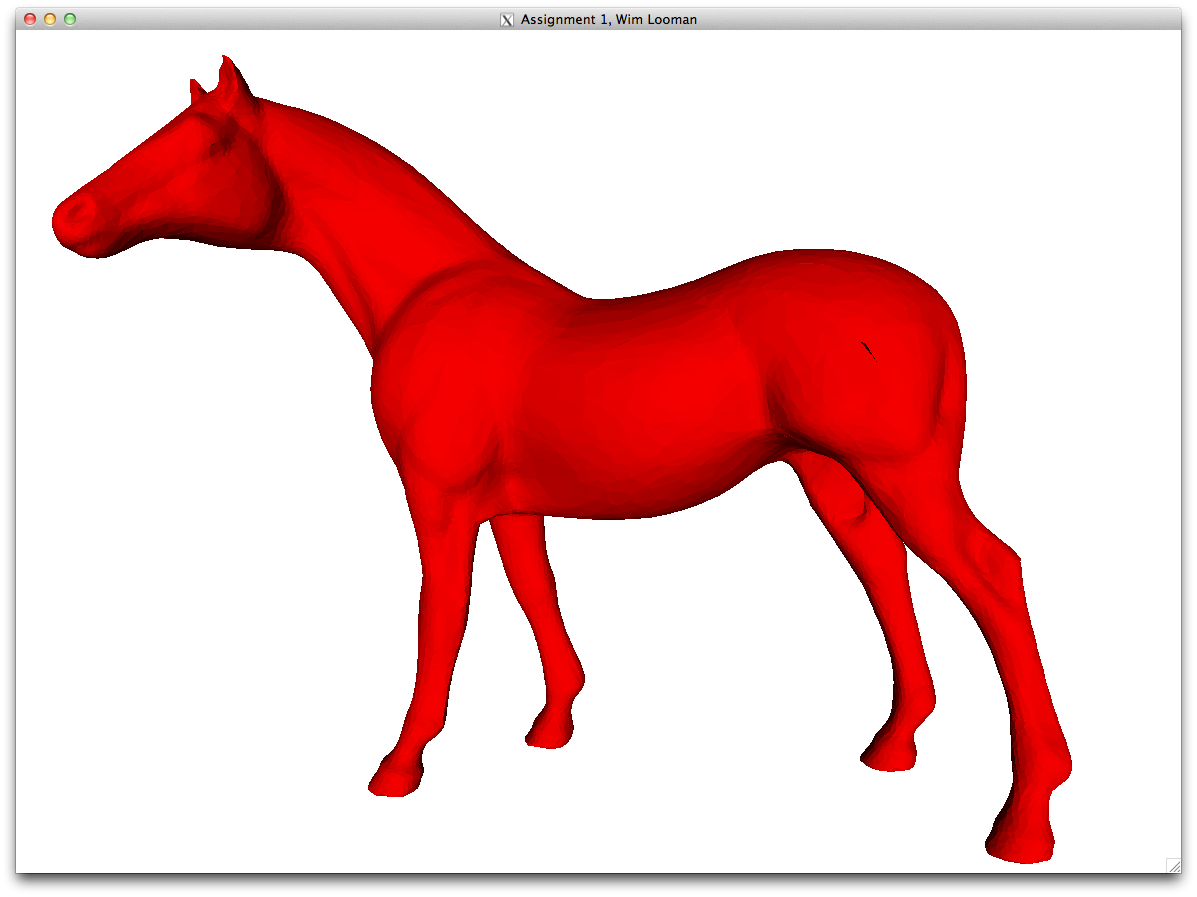
\includegraphics[width=0.35\textwidth]{images/Biowares_19848}
    }
    \\
    \subfloat[Simple Error Metric - 9922 polygons - 25\%]{
      \label{simple2}
      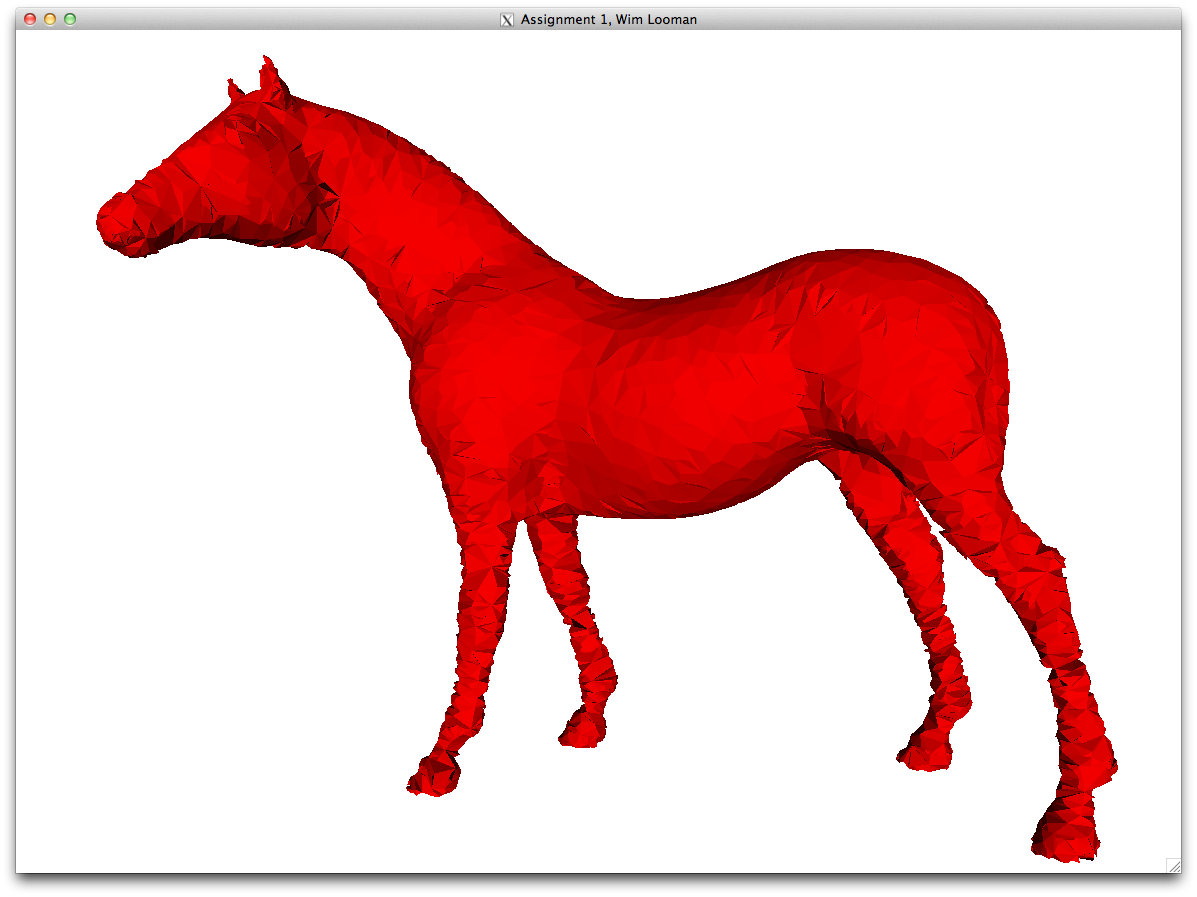
\includegraphics[width=0.35\textwidth]{images/Simple_9922}
    }
    \hspace{0.1\textwidth}
    \subfloat[Stan Melax's Error Metric - 9922 polygons - 25\%]{
      \label{melax2}
      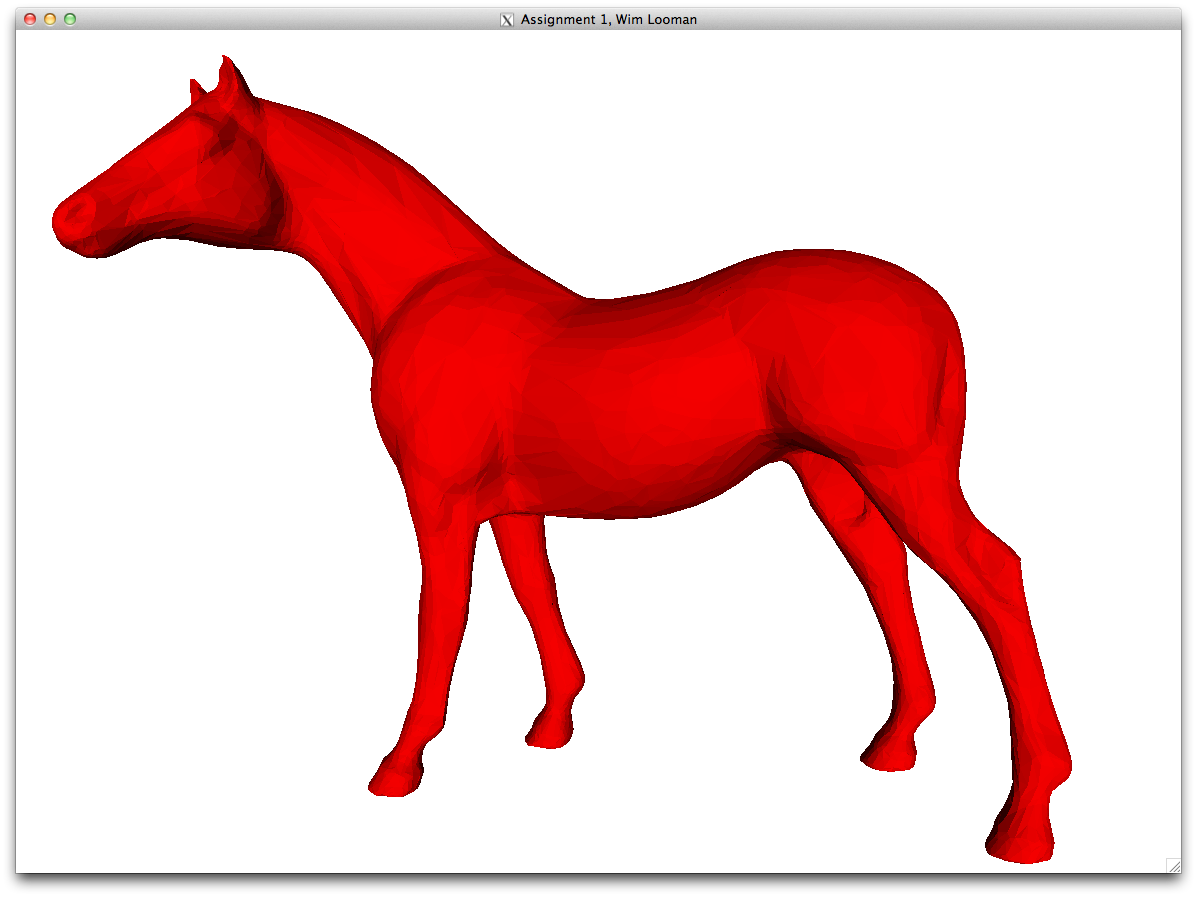
\includegraphics[width=0.35\textwidth]{images/Biowares_9922}
    }
    \\
    \subfloat[Simple Error Metric - 4960 polygons - 12.5\%]{
      \label{simple3}
      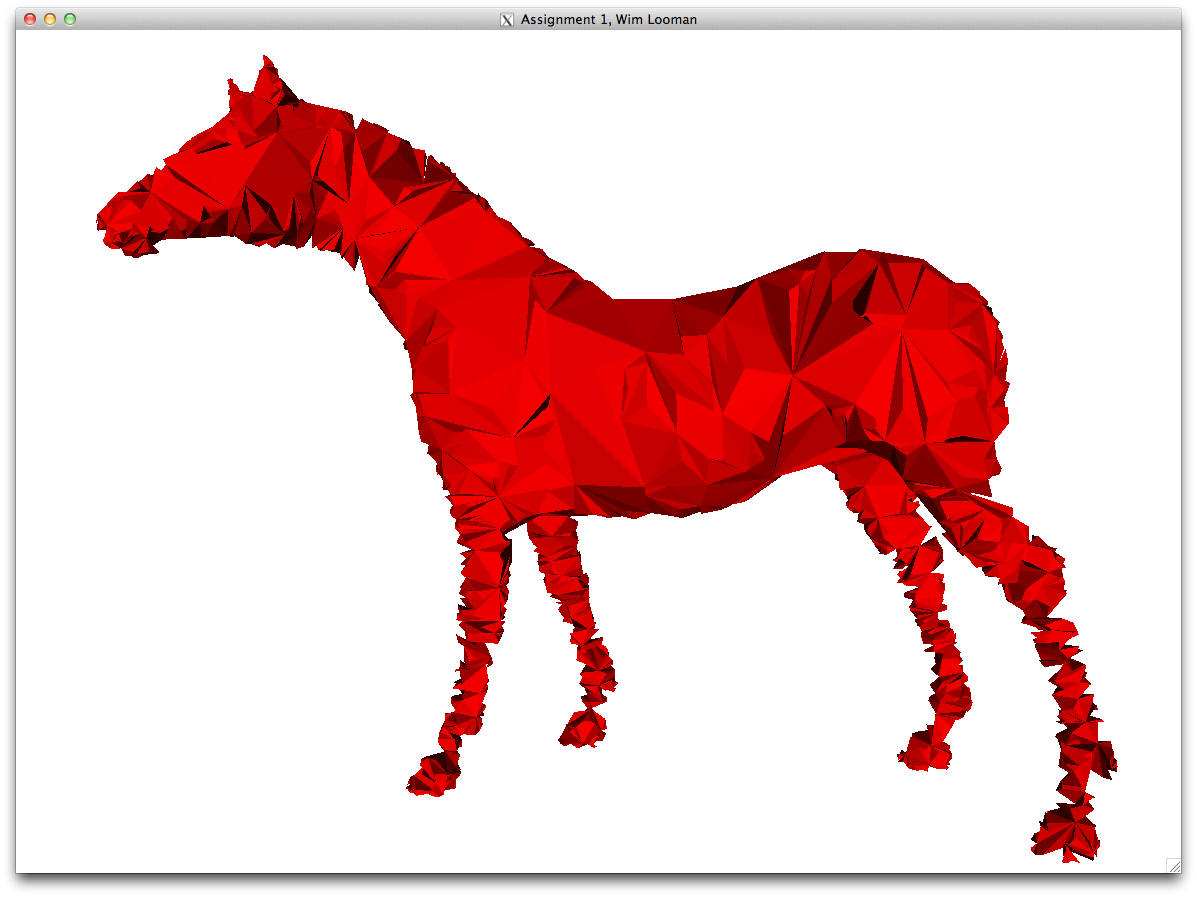
\includegraphics[width=0.35\textwidth]{images/Simple_4960}
    }
    \hspace{0.1\textwidth}
    \subfloat[Stan Melax's Error Metric - 4960 polygons - 12.5\%]{
      \label{melax3}
      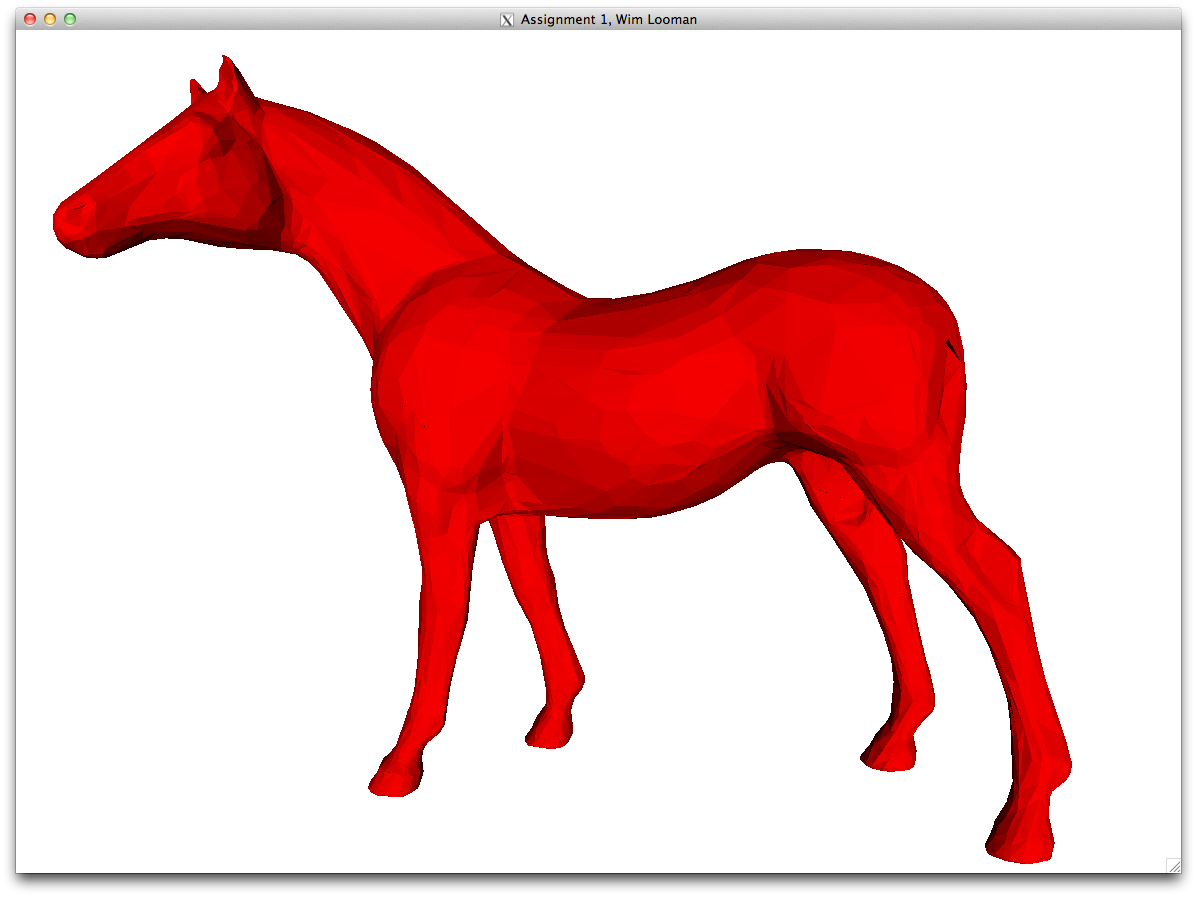
\includegraphics[width=0.35\textwidth]{images/Biowares_4960}
    }
    \caption{Comparison of the mesh simplification\label{simplification}}
  \end{figure}

  \begin{figure}
    \centering
    \subfloat[2478 polygons - 6.2\%]{
      \label{melax4}
      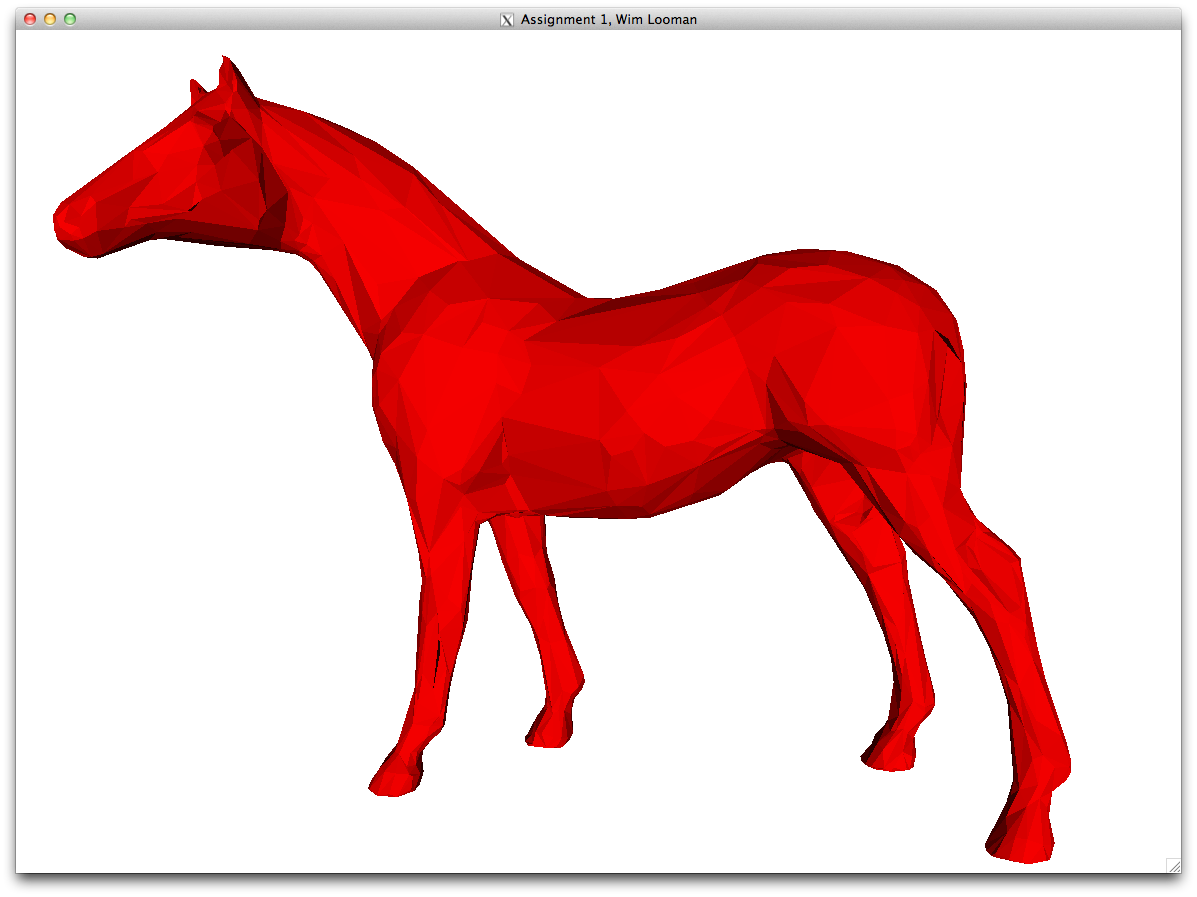
\includegraphics[width=0.35\textwidth]{images/Biowares_2478}
    }
    \hspace{0.1\textwidth}
    \subfloat[Normal mapped - 2478 polygons - 6.2\%]{
      \label{melax4w}
      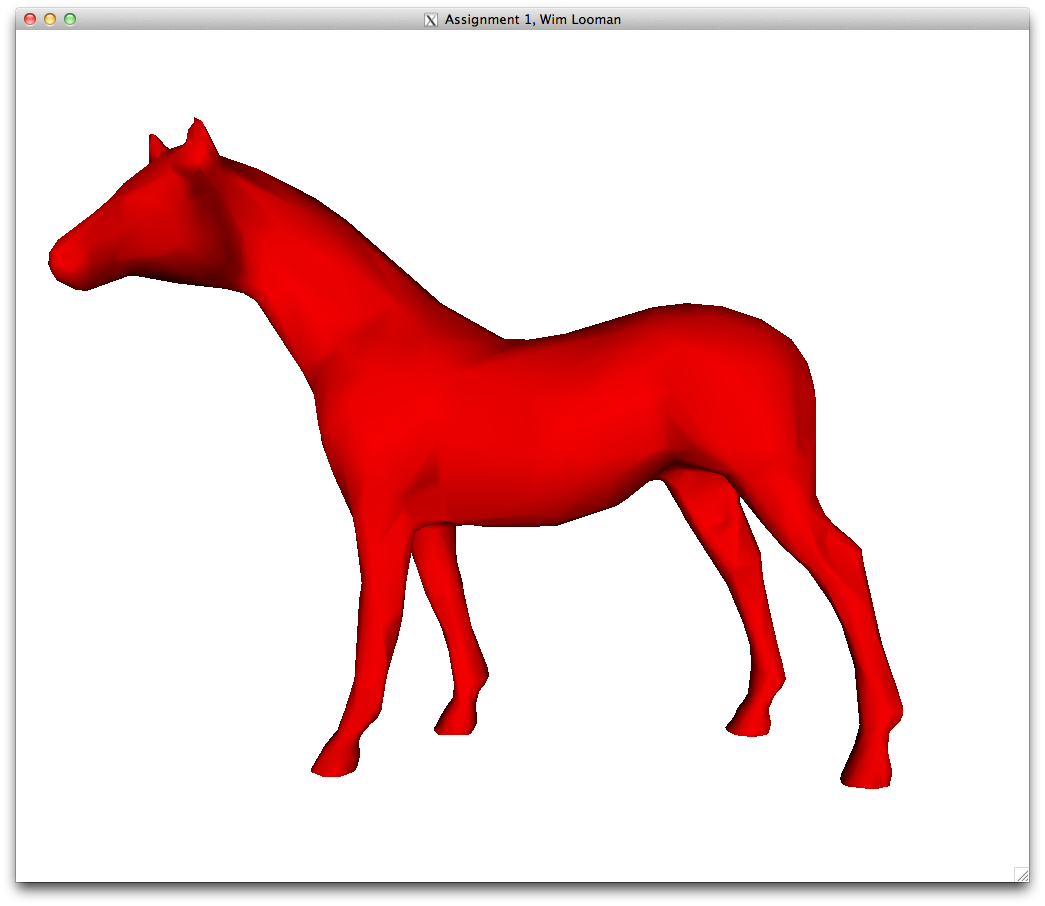
\includegraphics[width=0.35\textwidth]{images/Biowares_Smooth_2478}
    }
    \\
    \subfloat[618 polygons - 1.6\%]{
      \label{melax5}
      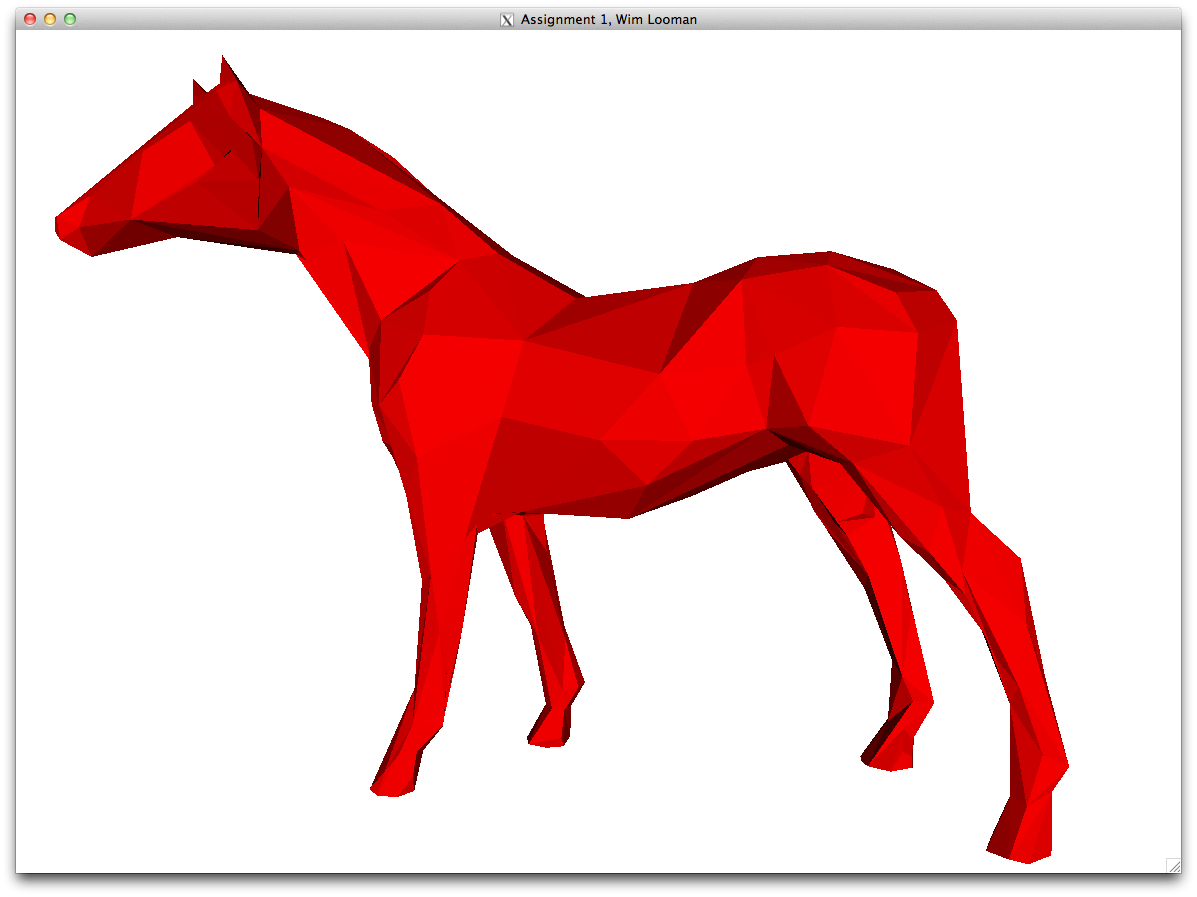
\includegraphics[width=0.35\textwidth]{images/Biowares_618}
    }
    \hspace{0.1\textwidth}
    \subfloat[Normal mapped - 618 polygons - 1.6\%]{
      \label{melax5w}
      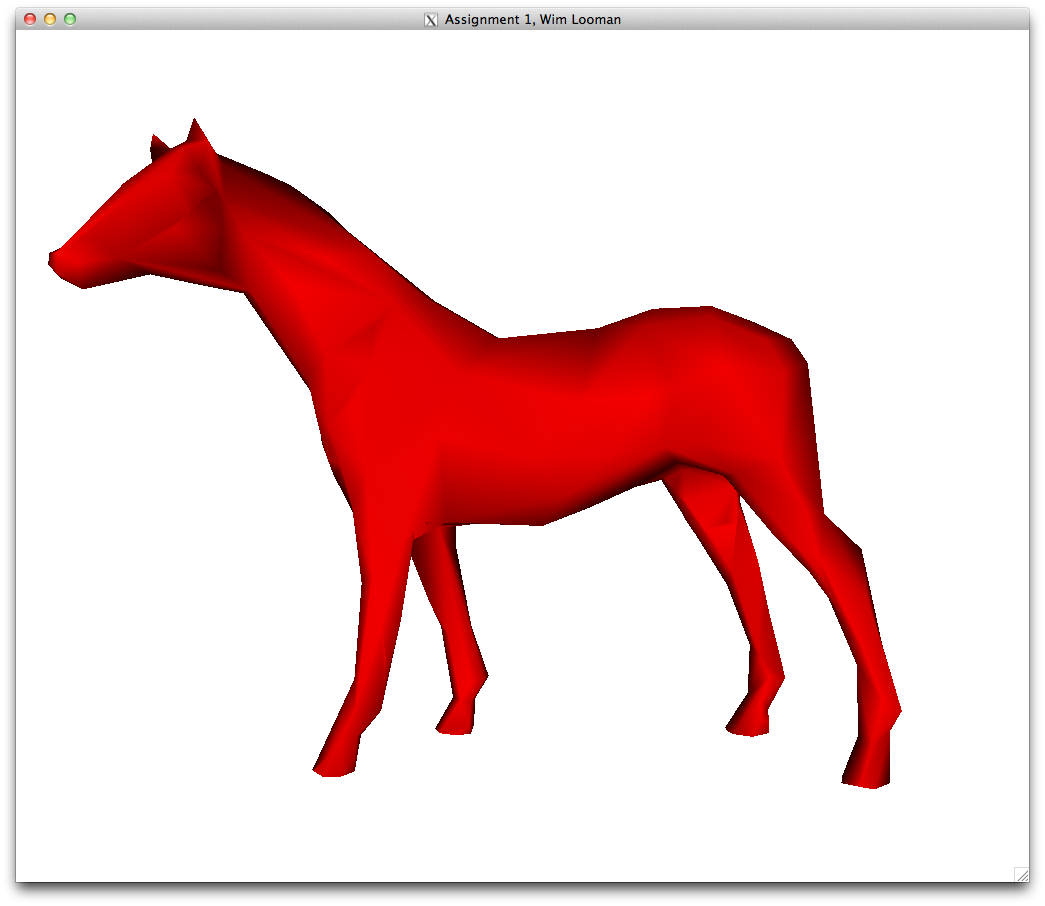
\includegraphics[width=0.35\textwidth]{images/Biowares_Smooth_618}
    }
    \\
    \subfloat[152 polygons - 0.4\%]{
      \label{melax6}
      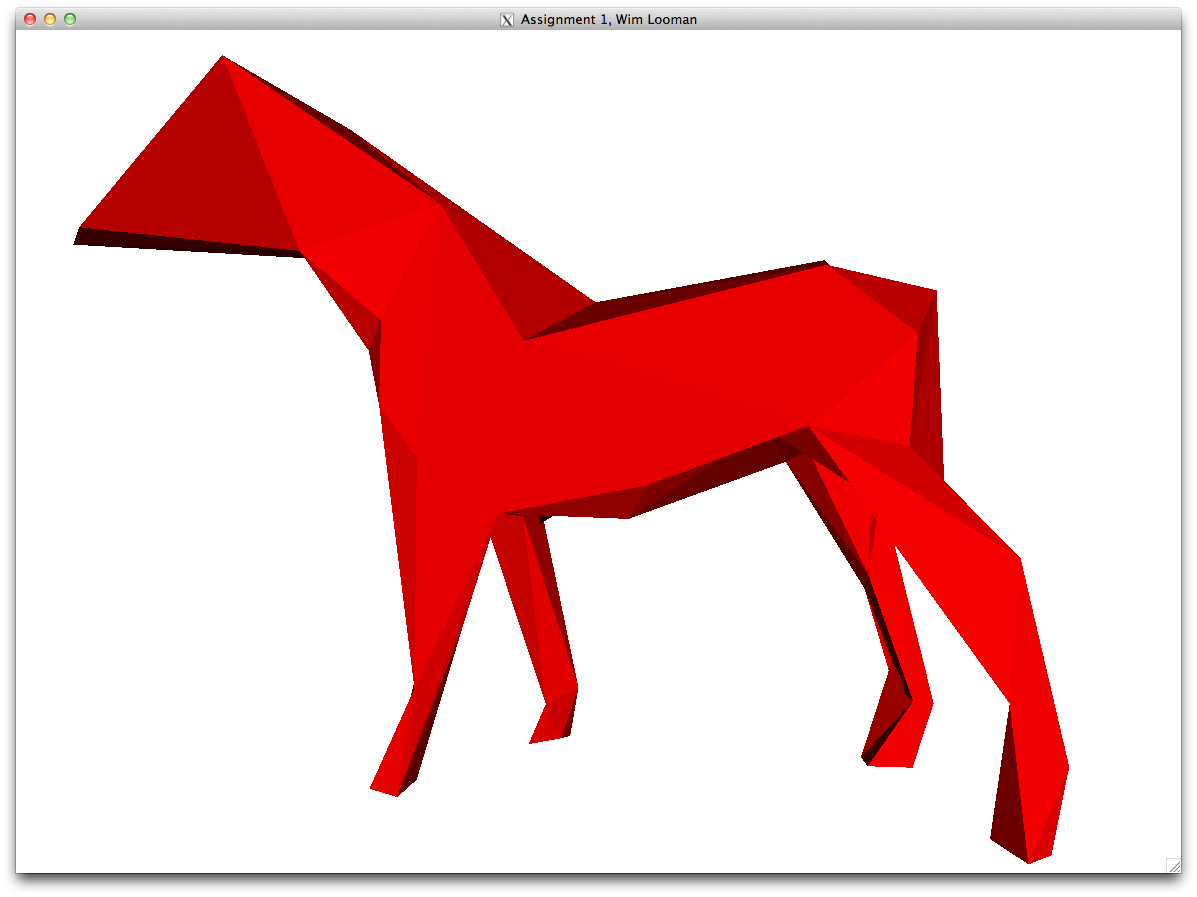
\includegraphics[width=0.35\textwidth]{images/Biowares_152}
    }
    \hspace{0.1\textwidth}
    \subfloat[Normal mapped - 152 polygons - 0.4\%]{
      \label{melax6w}
      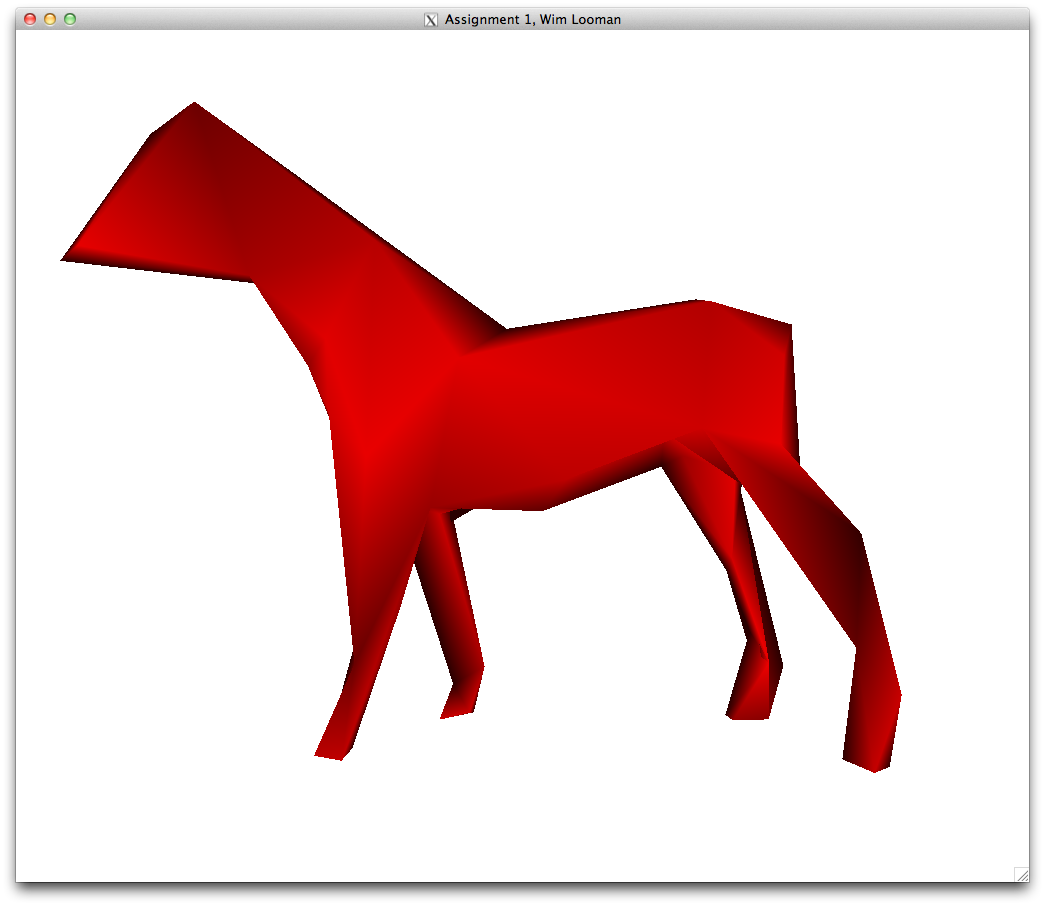
\includegraphics[width=0.35\textwidth]{images/Biowares_Smooth_152}
    }
    \caption{Extreme simplification with Stan Melax's Error Metric.\label{extreme}}
  \end{figure}
